\documentclass[tikz,border=0pt]{standalone}
\usepackage[utf8]{inputenc}
\usepackage[T1]{fontenc}
\usepackage{lmodern}
\usepackage{amsmath,amssymb}
\usetikzlibrary{arrows.meta,positioning,fit,calc,backgrounds,shapes.geometric,decorations.pathreplacing}
\definecolor{navy}{HTML}{163A5F}
\definecolor{blue}{HTML}{2C6EAF}
\definecolor{lightblue}{HTML}{EAF2F8}
\definecolor{midblue}{HTML}{CFE1F2}
\definecolor{graytext}{HTML}{4A5560}
\definecolor{lightgray}{HTML}{F4F6F8}
\definecolor{green}{HTML}{3C8D73}
\definecolor{lightgreen}{HTML}{E8F5EF}
\definecolor{red}{HTML}{B24A4A}
\definecolor{lightred}{HTML}{FBEDEE}
\tikzset{
  title/.style={font=\sffamily\bfseries\fontsize{16}{18}\selectfont,text=navy,anchor=west},
  subtitle/.style={font=\sffamily\bfseries\fontsize{11}{13}\selectfont,text=navy},
  body/.style={font=\sffamily\fontsize{9.2}{11}\selectfont,text=graytext,align=left},
  small/.style={font=\sffamily\fontsize{8}{9.4}\selectfont,text=graytext,align=left},
  tinylabel/.style={font=\sffamily\fontsize{7.2}{8.4}\selectfont,text=graytext},
  panel/.style={rounded corners=3pt,draw=midblue,fill=white,line width=0.6pt},
  box/.style={rounded corners=2pt,draw=midblue,fill=lightblue,line width=0.6pt},
  worker/.style={rounded corners=2pt,draw=blue,dashed,line width=0.7pt,fill=white},
  task/.style={rounded corners=2pt,draw=blue,fill=lightblue,minimum width=0.85cm,minimum height=0.55cm,font=\sffamily\bfseries\small,text=navy},
  file/.style={draw=blue,fill=white,minimum width=0.55cm,minimum height=0.42cm,font=\sffamily\small,text=navy},
  arr/.style={-{Stealth[length=2.4mm,width=1.8mm]},draw=blue,line width=0.9pt},
  arrthin/.style={-{Stealth[length=2mm,width=1.5mm]},draw=blue,line width=0.7pt},
  arrred/.style={-{Stealth[length=2mm,width=1.5mm]},draw=red,dashed,line width=0.8pt},
  arrgreen/.style={-{Stealth[length=2mm,width=1.5mm]},draw=green,dotted,line width=1pt}
}
\begin{document}

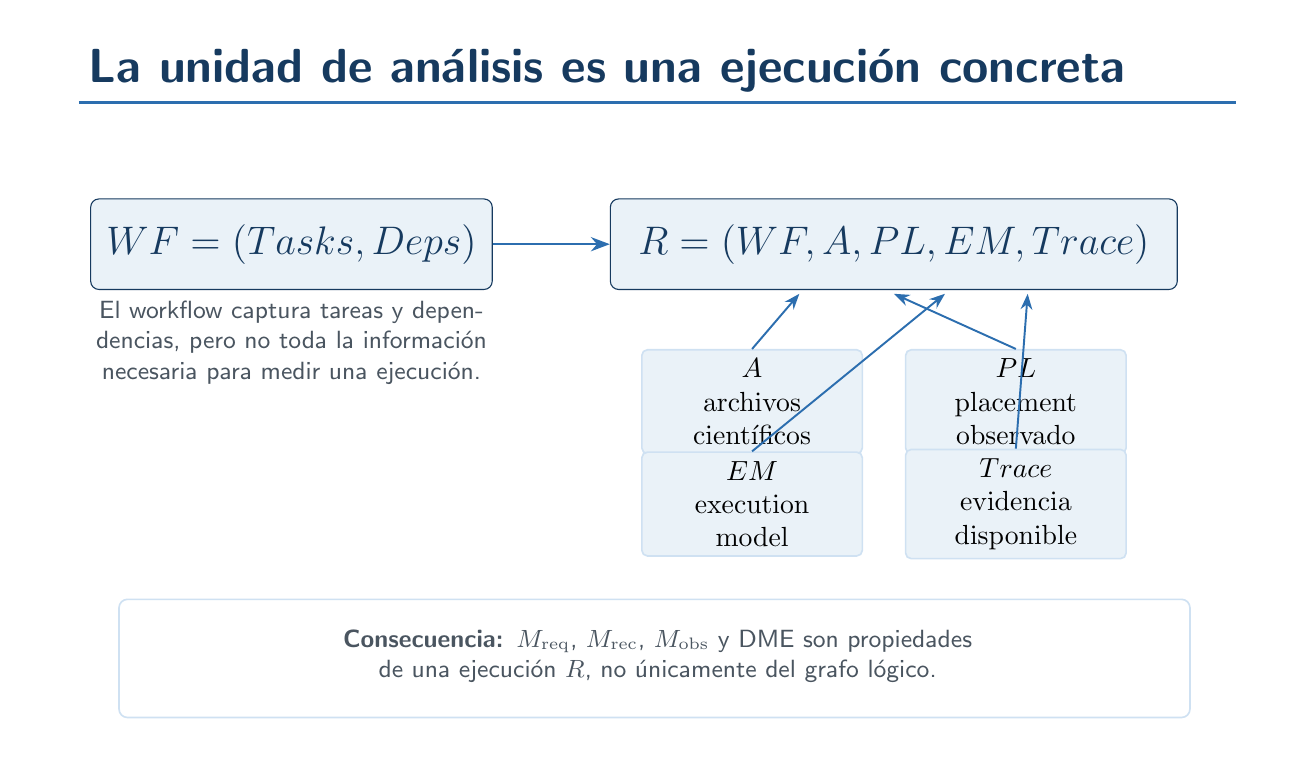
\begin{tikzpicture}[x=1cm,y=1cm]
\path[use as bounding box] (0,0) rectangle (16,9);
\node[title] at (0.65,8.45) {La unidad de análisis es una ejecución concreta};
\draw[blue,line width=1pt] (0.65,8.05)--(15.35,8.05);
\node[rounded corners=3pt,draw=navy,fill=lightblue,minimum width=5.1cm,minimum height=1.15cm,font=\sffamily\bfseries\Large,text=navy] (wf) at (3.35,6.25) {$WF=(Tasks,Deps)$};
\node[body,text width=5.4cm,align=center] at (3.35,5.0) {El workflow captura tareas y dependencias, pero no toda la información necesaria para medir una ejecución.};
\node[rounded corners=3pt,draw=navy,fill=lightblue,minimum width=7.2cm,minimum height=1.15cm,font=\sffamily\bfseries\Large,text=navy] (r) at (11.0,6.25) {$R=(WF,A,PL,EM,Trace)$};
\draw[arr] (wf)--(r);
\node[box,minimum width=2.8cm,minimum height=0.95cm,text width=2.45cm,align=center] (a) at (9.2,4.25) {\textbf{$A$}\\archivos científicos};
\node[box,minimum width=2.8cm,minimum height=0.95cm,text width=2.45cm,align=center] (pl) at (12.55,4.25) {\textbf{$PL$}\\placement observado};
\node[box,minimum width=2.8cm,minimum height=0.95cm,text width=2.45cm,align=center] (em) at (9.2,2.95) {\textbf{$EM$}\\execution model};
\node[box,minimum width=2.8cm,minimum height=0.95cm,text width=2.45cm,align=center] (tr) at (12.55,2.95) {\textbf{$Trace$}\\evidencia disponible};
\draw[arrthin] (a.north)--(9.8,5.62); \draw[arrthin] (pl.north)--(11.0,5.62); \draw[arrthin] (em.north)--(11.65,5.62); \draw[arrthin] (tr.north)--(12.7,5.62);
\node[panel,minimum width=13.6cm,minimum height=1.5cm,anchor=north west] at (1.15,1.75) {};
\node[body,text width=12.5cm,align=center] at (8,1.02) {\textbf{Consecuencia:} $M_{\mathrm{req}}$, $M_{\mathrm{rec}}$, $M_{\mathrm{obs}}$ y DME son propiedades de una ejecución $R$, no únicamente del grafo lógico.};
\end{tikzpicture}
\end{document}
